\section{Ergebnisse}
In dieser Arbeit wurden 14 unterschiedliche Knochentypen mit je vier verschiedenen Mess-Dimensionen über noch einmal 4 Zeitperioden betrachtet. 
Das sind 14 Diagramme mit je 4 Plots, die an dieser Stelle nicht alle einzeln ausgewertet werden können. 
Ich konzentriere mich daher in der Auswertung auf den Knochentyp »Metatarsal« und hier auf die Dimension »Bp«.
Alle anderen Plots und statistischen Auswertungen finden sich im Ordner \texttt{results}. 

\subsection{Grafische Darstellung der Daten}
Die nun vorbereiteten Daten lassen sich wunderbar in Form sogenannter »Raincloud Plots«\cite{Allen2021} darstellen. Raincloud Plots sind halbe Violin Plots, ergänzt durch einen Scatterplot der Rohdaten und einen Boxplot für eine einfache Übersicht der Mittelwerte und Ausreißer. 
Die Raincloud Plots wurden mit Hilfe des interaktiven Tutorials von \cite{Allen2021} erstellt, zu sehen im \texttt{ab\_plots.ipynb}.

\begin{figure}[H]
    \centering
    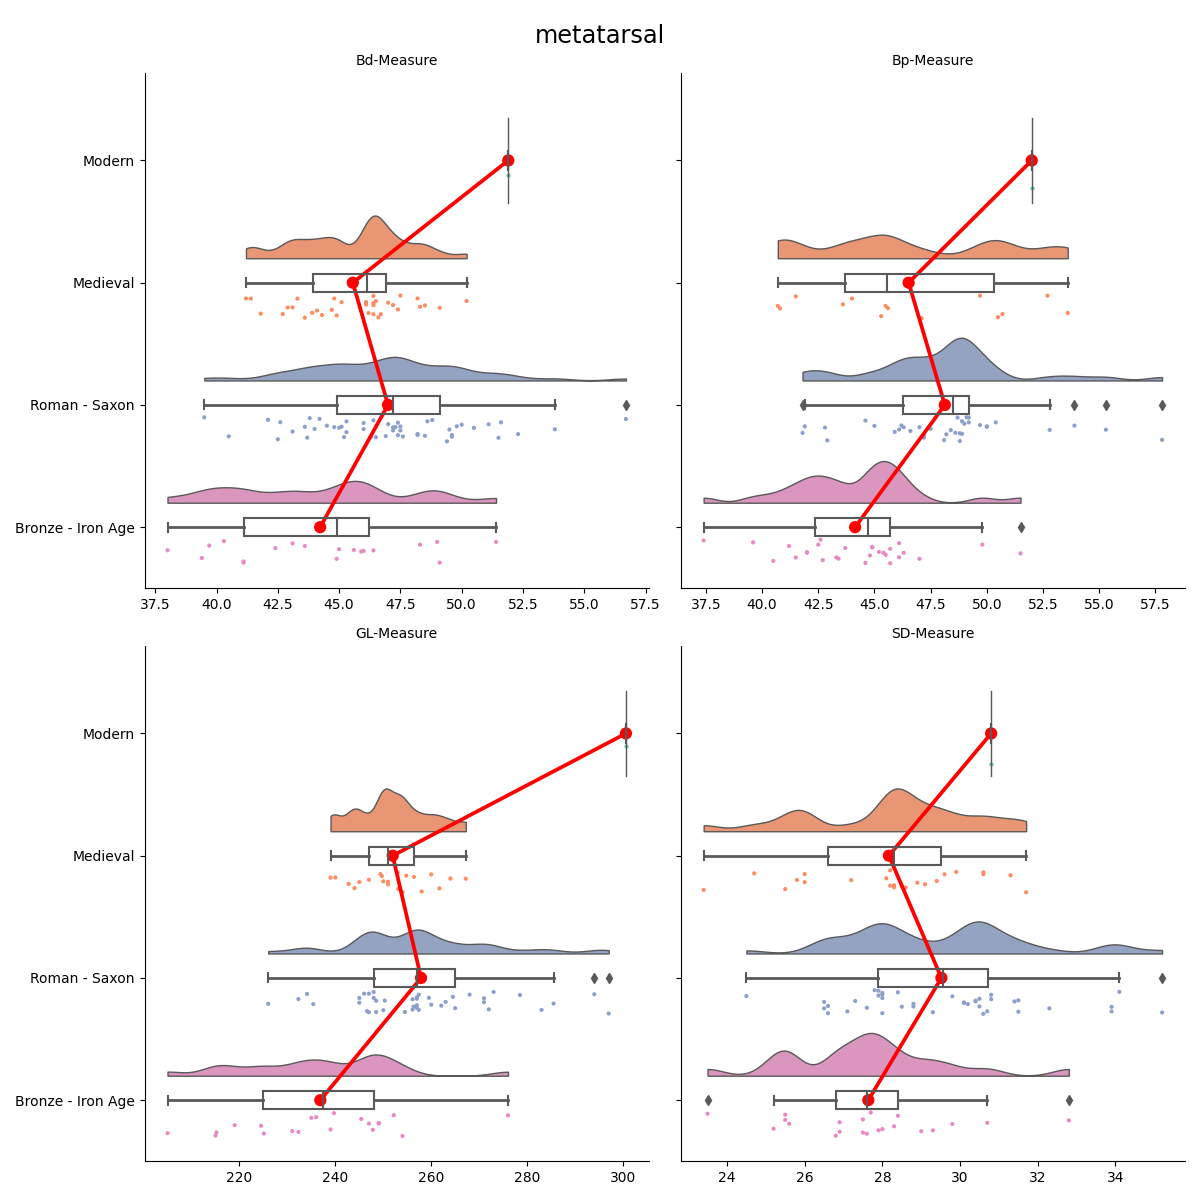
\includegraphics[height=10cm]{results/plots/rainclouds/metatarsal.png}
    \caption{Raincloud Plots für die Metatarsal Knochen}
    \label{fig:raincloud}
\end{figure}

An \autoref{fig:raincloud} lässt sich gut erkennen, dass die Knochengrößen sich bei allen Dimensionen zwischen den einzelnen Perioden unterscheiden. 
Im Intervall »Roman - Saxon« sind die Knochen in allen vier Dimensionen deutlich größer als sowohl zuvor in der Periode »Bronze - Iron Age« als auch später im »Medieval«. 
Von »Medieval« zu »Modern« nimmt die Größe bei allen vier Dimensionen wieder zu.

\subsection{Statistische Auswertung}
Um zu prüfen, ob die auf Grundlage des Plots aufgestellten Vermutungen statistisch relevant sind, wird ein Hypothesentest durchgeführt. 
Dazu werden Nullhypothese und Gegenhypothese aufgestellt: \\
$H_0$: Die absolute Datierung eines Knochens ist kein Indikator für dessen Größe.\\
$H_1$: Die absolute Datierung eines Knochens ist ein Indikator für dessen Größe.\\

Die Messdaten sind metrische Daten auf einer Verhältnisskala, die Perioden sind metrische Daten auf einer Intervallskala. 
Die Stichprobe ist unabhängig, da die Knochen aus jeder Periode distinkt sind - kein Knochen wurde zweimal für unterschiedliche Perioden datiert und hat auf dem Weg dorthin seine Größe verändert.
Um die Nullhypothese $H_0$ zu testen, wurde mit Hilfe von Welch's T-Test der p-Wert ermittelt und gegen das Signifikanz-Niveau von $\alpha = 0.05$ getestet. 
Ein p-Wert, der größer ist als $\alpha$ suggeriert, dass der Zusammenhang zwischen Datierung und Größe sehr wahrscheinlich zufällig ist. 
Ist der p-Wert hingegen kleiner als $\alpha$, kann die Nullhypothese abgelehnt und ein Zusammenhang zwischen Alter des Knochens und Größe als wahrscheinlich angenommen werden.
\begin{figure}[H]
    \centering
    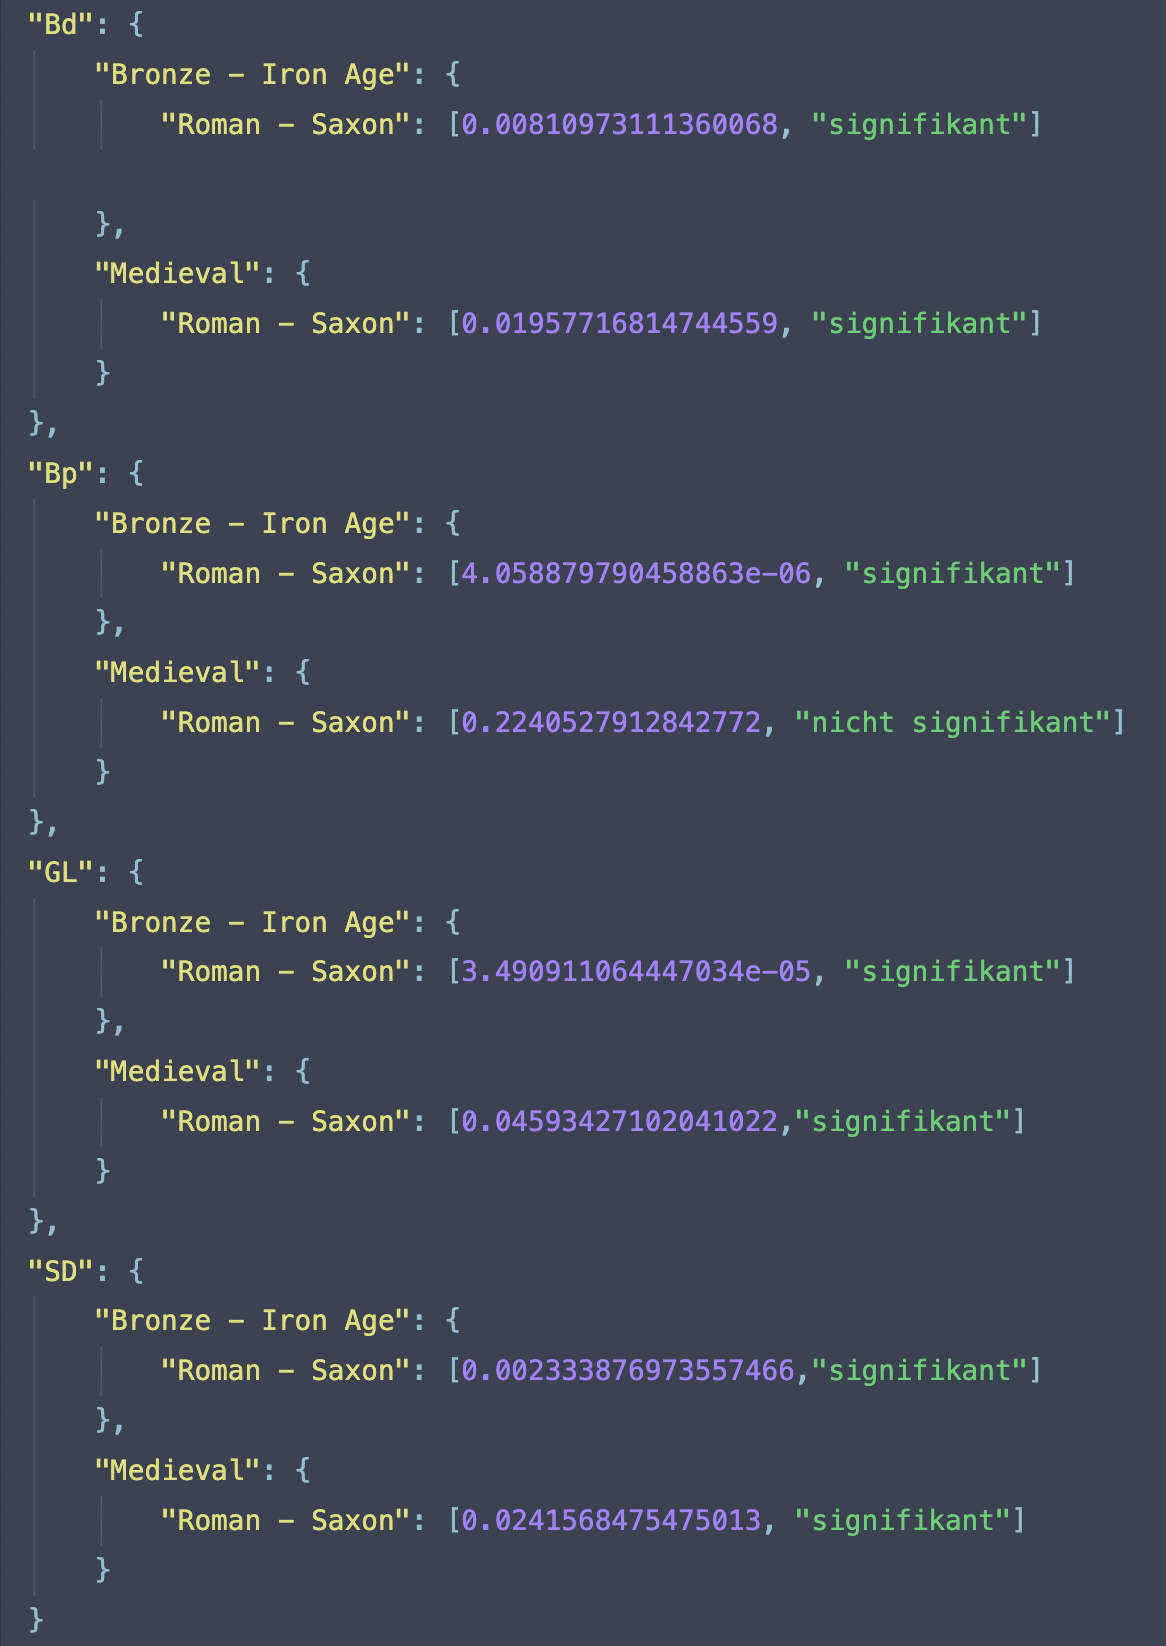
\includegraphics[height=10cm]{docs/latex/attachments/metatarsal_p-values.png}
    \caption{P-Werte für Metatarsal Knochengröße und Perioden}
    \label{fig:p-values}
\end{figure}

\autoref{fig:p-values} zeigt die p-Werte für die Metatarsal Knochen im Vergleich zwischen den relevanten Perioden.
Der Hypothesentest bestätigt, was zuvor bereits anhand des Raincloud Plots vermutet wurde: Die Größenunterschiede zwischen den einzelnen Perioden sind signifikant.
Der p-Wert ist für alle Vergleiche zwischen aufeinander folgenden Perioden signifikant.